\section{Hamiltonian Ising sebagai Representasi Sistem Kuantum}
Setiap sistem fisik yang perilakunya didorong oleh prinsip minimisasi energi dapat direpresentasikan ke dalam Hamiltonian operator secara universal, tidak terkecuali pada konfigurasi seleksi aset finansial yang memiliki kompleksitas variabel yang sangat tinggi. Dalam kerangka ekonofisika, proses pengambilan keputusan untuk alokasi portofolio strategis dipetakan ke dalam lanskap energi di mana solusi optimal secara teknis setara dengan konfigurasi energi terendah atau \textit{ground state} dari sistem tersebut \cite{lucas_ising_2014}. Pemetaan ini menganggap setiap instrumen investasi sebagai partikel \textit{spin} yang saling berinteraksi, di mana derajat korelasi antar pergerakan harga dimodelkan sebagai koefisien kopling di dalam sebuah kisi kristal yang terstruktur \cite{galam_ising_2010}. Representasi Hamiltonian Ising tersebut menyediakan jembatan teoretis antara optimasi kombinatorial klasik dengan perangkat keras kuantum yang memungkinkan penggunaan algoritma variasi untuk menavigasi ruang solusi berdimensi tinggi secara efisien \cite{hidalgo_quantum_2006}. Oleh karena itu, pemodelan sistem finansial sebagai sistem fisik memungkinkan analisis yang lebih ketat terhadap stabilitas pasar dan fenomena transisi fase melalui kacamata mekanika statistik yang telah mapan.

\subsection{Sejarah dan Evolusi Model Ising}
Model Ising secara historis dikonseptualisasikan oleh Wilhelm Lenz dan Ernst Ising pada awal dekade 1920-an sebagai instrumen teoretis revolusioner untuk menyelidiki asal-usul mikroskopis dari fenomena feromagnetisme \cite{niss_history_2005}. Fokus fundamental dari model ini terletak pada penyederhanaan interaksi fisik antara momen magnetik diskrit yang disusun dalam kisi reguler guna mengevaluasi munculnya keteraturan makroskopik dari fluktuasi termal lokal. Melalui pendekatan mekanika statistik, model ini berupaya menjawab pertanyaan krusial mengenai bagaimana orientasi mandiri dari partikel-partikel \textit{spin} yang saling bertetangga dapat memicu transisi fase sistemik pada suhu kritis tertentu. Keberhasilan awal dalam merumuskan kerangka kerja aksiomatik ini memberikan fondasi yang sangat kokoh bagi pengembangan teori fenomena kooperatif yang menjadi pilar utama dalam fisika statistik modern.

Meskipun memiliki landasan yang kuat, studi orisinal oleh Ernst Ising pada sistem satu dimensi (1D) menghasilkan kesimpulan pesimistis bahwa model tersebut tidak mampu mendemonstrasikan transisi fase pada suhu di atas nol mutlak. Analisis terhadap rantai interaksi biner berukuran hingga menunjukkan bahwa fluktuasi termal selalu mendominasi energi interaksi sehingga mencegah terbentuknya keteraturan magnetik yang stabil dalam skala makroskopik \cite{chamberlin_nanothermodynamics_2024}. Figure \ref{fig:1D_Ising} mengilustrasikan konfigurasi \textit{spin} pada model satu dimensi tersebut, di mana distribusi orientasi partikel cenderung bersifat acak akibat lemahnya korelasi jangka panjang pada dimensi yang rendah. Representasi visual ini merinci interaksi antar-partikel melalui tiga simbol utama, yaitu titik hitam ($\bullet$) untuk interaksi energi rendah, tanda silang ($\mathbf{X}$) untuk interaksi energi tinggi, serta lingkaran biru kosong (\textcolor{blue}{$\circ$}) sebagai pemutusan (\textit{break}) tanpa energi. Titik hitam merepresentasikan pasangan \textit{spin} paralel yang meminimalkan energi sistem, sedangkan tanda silang menunjukkan konfigurasi anti-paralel yang memicu peningkatan tegangan energi lokal \cite{chamberlin_nanothermodynamics_2024}. Lingkaran biru (\textcolor{blue}{$\circ$}) secara khusus menandai adanya pemutusan jalinan (\textit{subdivision}) yang memisahkan rantai menjadi subsistem independen guna mencapai kestabilan termal pada skala nanoskala. Pemetaan parameter interaksi mikroskopis ini memungkinkan pemodelan perilaku kolektif dan transisi fase pada sistem berukuran terbatas melalui perhitungan energi total yang mengombinasikan jumlah interaksi dan pemutusan tersebut secara sistematis.
\begin{figure}[htbp]
    \centering
    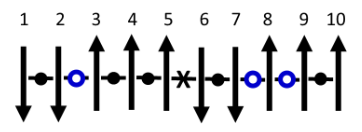
\includegraphics[width=0.7\textwidth]{Images/1D_Model_atT.png}
    \caption{Representasi visual model Ising satu dimensi (1D) yang menunjukkan dinamika orientasi \textit{spin} dan klasifikasi energi interaksi ($\bullet$, $\mathbf{X}$, \textcolor{blue}{$\circ$}) di bawah pengaruh fluktuasi termal \cite{chamberlin_nanothermodynamics_2024}.}
    \label{fig:1D_Ising}
\end{figure}
Kekakuan hasil matematis pada dimensi tunggal ini sempat memicu skeptisisme terhadap relevansi fisik model Ising, sebelum akhirnya paradigma tersebut berubah total setelah Lars Onsager merumuskan solusi eksak untuk kasus dua dimensi yang sangat kompleks.

Kebangkitan minat terhadap model Ising terjadi pada era 1930-an hingga 1940-an setelah para fisikawan menyadari kapasitas model tersebut dalam merepresentasikan berbagai fenomena kooperatif di luar bidang magnetisme \cite{niss_history_2005}. Struktur energi yang dibentuk oleh interaksi antar \textit{spin} ternyata memiliki kemiripan topologi dengan berbagai masalah optimasi kombinatorial yang ditemukan dalam sistem biologis, kimia, maupun ekonomi global. Penemuan Lars Onsager mengenai transisi fase pada sistem dua dimensi membuktikan bahwa interaksi jarak pendek yang sederhana mampu menghasilkan perilaku kolektif yang sangat kaya dan tidak terduga. Saat ini, model Ising telah bertransformasi menjadi bahasa standar dalam ranah \textit{Ising Computing} yang menghubungkan masalah optimasi dunia nyata dengan arsitektur komputer kuantum berbasis \textit{Quantum Annealing} \cite{lucas_ising_2014}. Pendekatan ini memungkinkan penanganan kompleksitas ruang solusi yang tumbuh secara eksponensial melalui pemetaan parameter Hamiltonian yang presisi dan efisien pada perangkat keras mutakhir.

\subsection{Representasi Fisik Aset Finansial}
Dalam bidang ekonofisika, para agen ekonomi dianalogikan sebagai sistem partikel diskrit yang saling berinteraksi secara dinamis guna mencapai titik kesetimbangan energi yang paling stabil di tengah fluktuasi pasar. Setiap aset dalam portofolio investasi kemudian direpresentasikan sebagai entitas fisik \textit{spin} ($s_i$) yang memiliki dua arah keadaan tetap di dalam ruang Hilbert yang terdefinisi secara matematis \cite{galam_ising_2010}. Berdasarkan transformasi variabel yang digunakan, keadaan $-1$ merepresentasikan posisi beli (\textit{long}), sementara keadaan $+1$ digunakan untuk merepresentasikan posisi jual (\textit{short}) atau pengabaian aset dalam strategi alokasi modal \cite{lucas_ising_2014}. Representasi fisik ini memungkinkan analisis mendalam terhadap munculnya tren makroskopik pasar yang didasarkan pada akumulasi keputusan mikroskopik individu yang terekam dalam bentuk konfigurasi energi sistem. Interaksi antar \textit{spin} tersebut ditentukan oleh kekuatan korelasi yang dimiliki masing-masing aset melalui data ekspektasi imbal hasil dan matriks kovarians yang telah diperoleh sebelumnya \cite{hidalgo_quantum_2006}.

Perilaku kolektif yang terjadi di pasar finansial, seperti fenomena korelasi harga antar instrumen, dapat dianalogikan sebagai interaksi magnetik antar partikel dalam sebuah kisi kristal yang terstruktur \cite{galam_ising_2010}. Secara fisik, hubungan korelasi ini setara dengan parameter \textit{coupling} ($J_{ij}$), di mana kekuatan interaksi tersebut menentukan kecenderungan setiap \textit{spin} untuk menyelaraskan arah orientasinya terhadap tetangganya. Sementara itu, ekspektasi imbal hasil dari setiap aset berperan sebagai medan magnet eksternal (\textit{external field}) yang memberikan dorongan kuat pada arah orientasi \textit{spin} tertentu guna memaksimalkan utilitas investasi \cite{lucas_ising_2014}. Hamiltonian sistem kemudian digunakan untuk menghitung total energi yang merepresentasikan total konflik atau ketidakstabilan strategi investasi, di mana nilai energi minimum menjadi indikator utama dari solusi portofolio yang paling optimal. Integrasi antara parameter ekonomi dan variabel fisik ini menciptakan sebuah ekosistem simulasi yang mampu merefleksikan dinamika pasar finansial secara akurat melalui pendekatan mekanika statistik yang ketat \cite{hidalgo_quantum_2006}.

\subsection{Pemetaan Kuantum: QUBO ke \textit{Pauli-Z}}
Transisi operasional dari domain optimasi biner klasik menuju arsitektur komputasi kuantum mensyaratkan transformasi variabel keputusan $x_i$ menjadi operator mekanika kuantum yang dapat diproses oleh \textit{qubit} di dalam sirkuit terpadu \cite{lucas_ising_2014}. Variabel biner tersebut secara eksplisit dipetakan ke dalam operator \textit{Pauli-Z} ($\hat{Z}_i$) melalui transformasi linear guna menjaga integritas logika masalah yang nilai eigennya merepresentasikan status basis komputasi $|0\rangle$ dan $|1\rangle$. Penurunan parameter fisik dilakukan melalui substitusi variabel $x_i = (1 - \sigma_i)/2$ yang menghasilkan rumusan medan lokal ($h_i$) serta kekuatan interaksi ($J_{ij}$) guna mengakomodasi prinsip minimisasi energi pada perangkat keras kuantum \cite{fedorov_vqe_2022}. Pemetaan ini menjamin bahwa setiap interaksi kovarians antar aset dapat diterjemahkan menjadi korelasi fase antar \textit{qubit} yang saling terikat secara kuantum di dalam lanskap energi sirkuit optimasi. Secara formal, Hamiltonian Ising yang merepresentasikan risiko portofolio tersebut dinyatakan melalui rumusan negatif pada kedua sukunya guna menyelaraskan antara maksimisasi utilitas finansial dengan minimisasi energi fisik sebagai berikut:
\begin{equation}
\hat{H} = - \sum_{i} h_i \hat{Z}_i - \sum_{i < j} J_{ij} \hat{Z}_i \hat{Z}_j
\end{equation}

Dengan konfigurasi Hamiltonian yang telah berhasil dipetakan secara akurat, algoritma \textit{Variational Quantum Eigensolver} (VQE) kemudian diimplementasikan untuk mencari solusi \textit{ground state} yang merepresentasikan alokasi aset paling optimal \cite{wang_variational_2025}. Algoritma hibrida ini bekerja dengan cara mengoptimalkan parameter sirkuit secara iteratif melalui kontrol klasik guna meminimalkan nilai ekspektasi energi dari Hamiltonian Ising yang telah dikonstruksi secara teknis \cite{fedorov_vqe_2022}. Implementasi inisialisasi cerdas melalui kerangka kerja \textit{Exact Potential Game} menjadi sangat esensial untuk memitigasi risiko kegagalan konvergensi akibat fenomena \textit{Barren Plateaus} pada perangkat keras \textit{Noisy Intermediate-Scale Quantum} (NISQ) \cite{mcclean_barren_2018, preskill_quantum_2018}. Keberhasilan proses optimasi ini menjamin bahwa setiap hasil pengukuran akhir pada \textit{qubit} memiliki interpretasi ekonomi yang sah dan logis sehingga memberikan keunggulan kompetitif dalam pengambilan keputusan investasi strategis. Integrasi antara logika teori permainan dan komputasi kuantum tersebut pada akhirnya menyediakan solusi yang lebih presisi dan stabil dalam menghadapi tantangan optimasi finansial yang bersifat \textit{NP-hard}.
